\documentclass[../report.tex]{subfiles}
\begin{document}
\graphicspath{{img/}{../img/}}

\section{The Waterfall Model}

Vandfaldsmodellen er en procesmodel hvor man besk�ftiger sig med forskellige faser, en ad gangen indtil man er n�et til slutningen af projektforl�bet. Denne model er ogs� kendt som one-shot eller once-through modellen, p� grund af dens ikke-iterative workflow. Modellen findes i forskellige udgaver, men den best�r ofte af fem predefinerede faser; \textit{Kravspecifikation}, \textit{Design}, \textit{Implementering}, \textit{Verificering} og \textit{Vedligeholdelse}.  

%The waterfall model is a process model which follows a sequence of phases working from the top to the bottom. It is also known as the one-shot or once-through model, because of the non-iterative workflow. The model exists in different versions, but it often consists of five predefined phases. That is \textit{Requirements}, \textit{Design}, \textit{Implementation}, \textit{Verification} and \textit{Maintenance}.

\begin{figure}[H]
\centering
	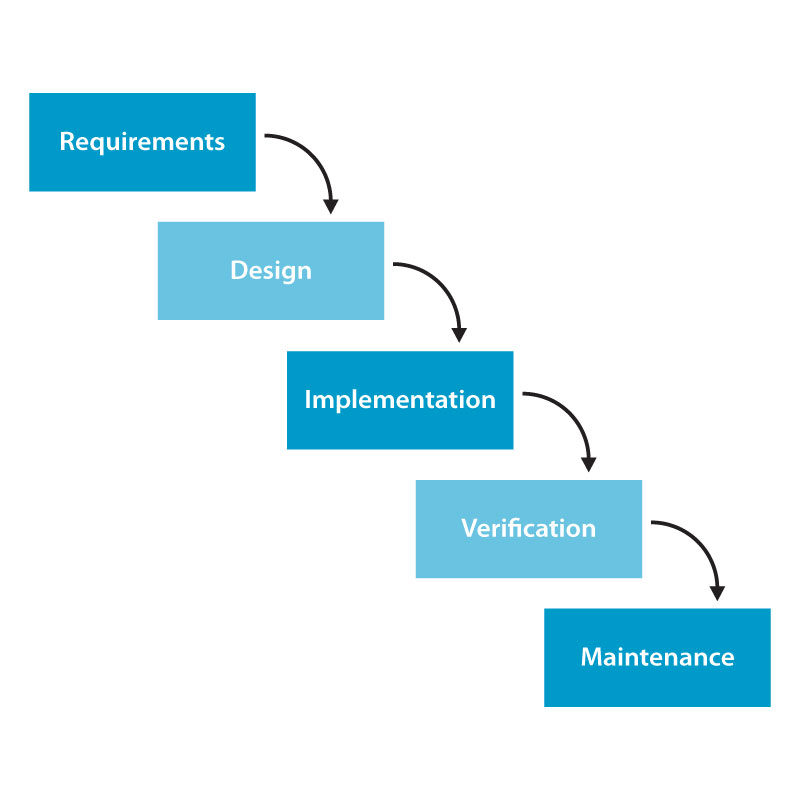
\includegraphics[scale=0.3]{h4_waterfall.jpg}
\caption{Vandfaldsmodellen}
\end{figure}

Retningen hvormed man arbejder med faserne skal altid v�re fremadg�ende eller nedadg�ende set i forhold til modellens analogi. Det er dog tiladt at ``plaske'' sig tilbage til den forrige fase, selvom dette er en undtagelse.

%The flow of the model should always be downwards, however the possibility of ``splashing'' back to the previous phase is allowed. This is more the exception than the rule.

\subsection{Strengths \& Weaknesses}
Det stringente workflow som denne model indholder giver begr�nsede muligheder for at iterere undervejs i projektet. Dette kan v�re en klar fordel, hvis kriterierne for projektet er veldefinerede og fastlagte fra start. Det er nemt at f�lge projektets udvikling undervejs b�de for udviklere, projektledere og for klienten, da hver fase naturligt genererer en milep�l for projektet. Dette betyder ogs� at det er nemt at evaluere p� den nyligt afsluttede fase samt at estimere hvor meget der pr�cist mangler f�r at projektet kan afsluttes.

%The strict flow of this process model gives a very limited scope for iteration. This limited scope is indeed a strength, if the requirements of the project are well defined. The progress of the project is easy to follow, both for developers, project managers and the client, since the end of each phase generates a natural milestone for the project. Because of this it is easy to evaluate on the current progress and estimation of the remainder of the project after each phase.

Vandfaldsmodellen er, som sagt, at foretr�kke hvis kriterierne for projektet er veldefinerede fra begyndelsen, samt at der ikke tilf�jes flere kriterier undervejs i processen. P� grund af den ikke-iterative arbejdsgang, er det ikke muligt at implementere nye kriterier undervejs. Modellen er generelt ufleksibel, da hver phase er fastlagt p� forh�nd.

%As said The Waterfall Model is preferred if the requirements are well defined, and that no more requirements will be added on later in the process. Because of the non-iterative workflow, there is no way to implement new requirements along the way, it is simply not allowed. The model is generally inflexible, due to the permanent dealings for each phase.
 
En anden ulempe ved modellen kunne v�re integrationen af produktet og muligheden for at klienten kan pr�ve produktet undervejs i forl�bet.

%Another weakness would be the integration of the product, and the possibility for the client to try the product during the project.

\end{document}